\documentclass[margin=10pt]{standalone}
\usepackage{color,xcolor}
\usepackage{makecell}
\usepackage{tikz-qtree, tikz}
\usepackage[utf8]{inputenc}
% trim={<left> <lower> <right> <upper>}
\begin{document}
\begin{tikzpicture}
    \node[anchor=south west,inner sep=0] (graph) at (0,0) {
        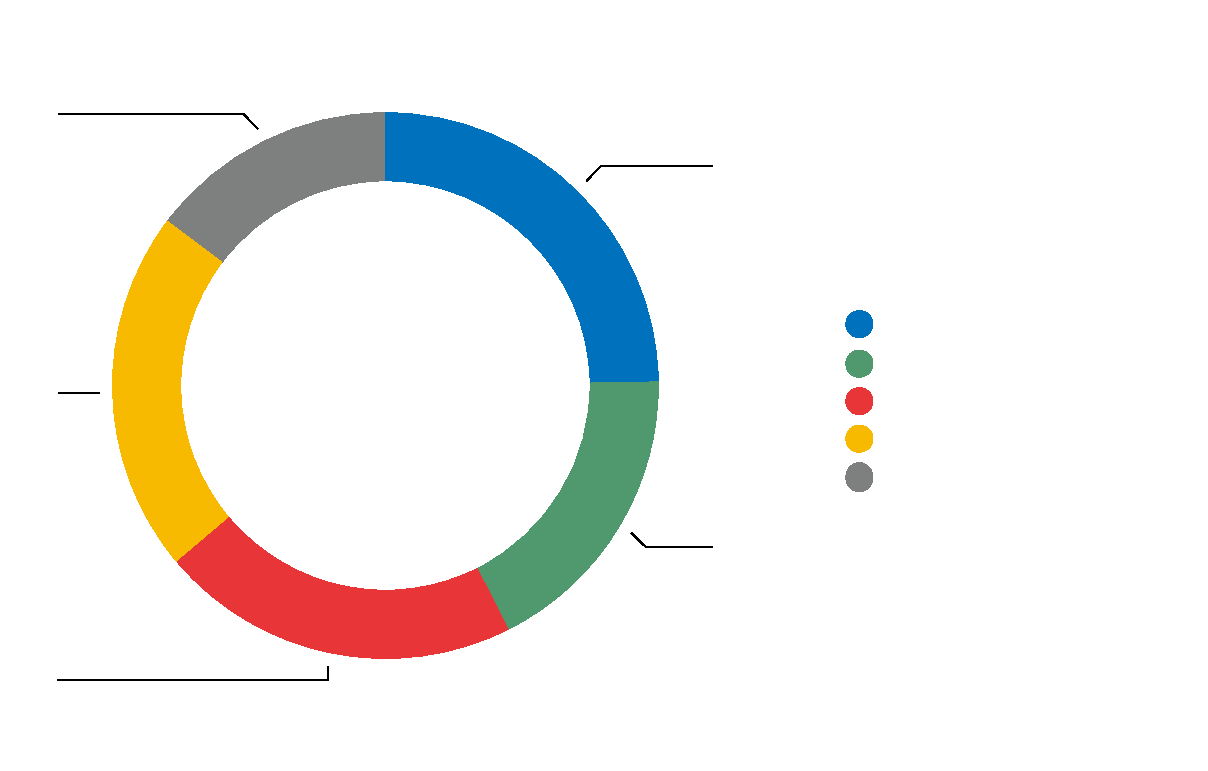
\includegraphics{domain-donut-chart-cropped.pdf}
    };
    \begin{scope}[x={(graph.south east)},y={(graph.north west)}]
        \node[black,anchor=west] (biomed) at (0.73,0.582){\Large Biomedical};
        \node[black,anchor=west] (auto) at (0.73,0.527){\Large Automotive/Aerospace};
        \node[black,anchor=west] (indus) at (0.73,0.482){\Large Industrial};
        \node[black,anchor=west] (bio) at (0.73,0.429){\Large Bio-Inspired};
        \node[black,anchor=west] (bio) at (0.73,0.382){\Large Others};

        \node[black,anchor=west] (bm) at (0.6,0.785){\Large $25\%$};
        \node[black,anchor=west] (bm) at (0.6,0.295){\Large $18\%$};
        \node[black,anchor=west] (bm) at (-0.015,0.855){\Large $15\%$};
        \node[black,anchor=west] (bm) at (-0.015,0.49){\Large $21\%$};
        \node[black,anchor=west] (bm) at (-0.015,0.12){\Large $21\%$};
    \end{scope}
\end{tikzpicture}
\end{document}
